\documentclass{article}
\usepackage[utf8]{inputenc}
\usepackage{geometry}
\usepackage{graphicx}
\usepackage{url,hyperref}
\usepackage{array}

\hypersetup{colorlinks,citecolor=red,urlcolor=blue} 
\newcolumntype{P}[1]{>{\raggedleft\arraybackslash}p{#1}}

\title{
	Web Information Extraction and Retrieval\\
	Programming Assignment 1: \\
	Crawler implementation
}

\author{
  Marko Prelevikj\\
  63130345\\
  \texttt{mp2638@student.uni-lj.si}
  \and
  Gojko Hajduković\\
  63180431\\
  \texttt{gh8590@student.uni-lj.si}
  \and
  Stefan Ivanišević\\
  63170405\\
  \texttt{si0539@student.uni-lj.si}
}
\date{April 2019}

\begin{document}

\maketitle

\section{Introduction}

\section{Implementation specifics}

The implementation of the web crawler is done in Scala, which is a functional programming language, offering a lot of syntactical sugars which make the development process easier.
We chose it in order to improve our programming skills in Scala, and also, learn a lot about its capabilities for concurrent programming.

\subsection{Dependencies}

To make the development process as easy as possible, we are using a number of dependencies. In this report, we are listing the once which are most significant, whilst the list of entire dependencies is available in the \texttt{build.sbt} file. 
\begin{itemize}
	\item \texttt{akka-actor} - providing us with the support of multi-threading through the concept of actor systems~\cite{Akka:ActorSystem}.
	\item \texttt{slick} - a functional relational mapping library to easily store data into the database~\cite{Slick}.
	\item \texttt{crawler-commons} - a library containing common utilities for crawlers~\cite{Crawler-commons}.
	\item \texttt{htmlunit} - headless browser which renders the html content of a provided URL~\cite{htmlunit}.
	\item \texttt{bigqueue} - a multithread-safe persistent queue for keeping the frontier~\cite{bigqueue}.
	\item \texttt{JSoup} - a library for HTML document parsing~\cite{jsoup}.
\end{itemize}

\subsection{Database modifications}

In order to make the implementation more insightful, we expanded the initial database with additional columns as follows:
\subsubsection{Table \texttt{page}}
We introduced the fields:
\begin{itemize}
    \item \texttt{hash} - SHA256 hash of the entire HTML content of the page, used for duplicate detection.
    \item \texttt{load\_time} - time needed to load the page
    \item \texttt{stored\_time} - when the page was added in the queue
\end{itemize}
\subsubsection{Table \texttt{page\_type}}
We introduced the following values:
\begin{itemize}
    \item \texttt{INVALID} - in case there has occurred an unknown error while loading the page
    \item \texttt{DISALLOWED} - if the page is not allowed by the \texttt{robots.txt} file
\end{itemize}

\subsubsection{Table \texttt{page\_data}}
We introduced the following column:
\begin{itemize}
    \item \texttt{filename} - canonical url of the stored file
\end{itemize}

\subsubsection{Storing process}

We altered the storing process as well. We omit a page entry of the type \textit{BINARY} which should be a reference to the \textit{image} or \textit{page\_data} table. Instead, we are linking the resources directly to the pages where they occurred. For example, if there had been an image linked to a page with \texttt{id = 1}, we enter an image entry with a reference to the page with \texttt{id = 1}.

\section{Crawler implementation}

The development process of the crawler was done in multiple iterations. In the first iteration, we developed all the required utilities to build the crawler upon. These utilities include: URL-canonicalization, \texttt{SiteMap} parsing, \texttt{robots.txt} parsing, database service to store the obtained data. Furthermore, we developed the core concepts, and the basic pipeline of how the crawler should interact with the frontier and the database. Finally, we created workers which are going to perform the crawling.

There are two versions of the crawler workers. First, we tried a naive implementation in~\ref{subsec:jitter} with jittered time between the requests to the same domain, which didn't turn out well. Next, we developed a more advanced version of the worker in~\ref{subsec:bf}, which implements a distributed breadth-first approach.

\subsection{Core concepts}

The following steps describe the process of fetching and storing the data retrieved from a given URL. Whenever we refer to processing of a page, we are referring to the following steps:
\begin{enumerate}
	\item frontier dequeueing - get the next page from the frontier
	\item \texttt{robots.txt} check - check whether the page is allowed in the \texttt{robots.txt}, skip it if not. If the \texttt{robots.txt} is missing - allow it by default
	\item page rendering - get the page content and HTTP status code using \texttt{HtmlUnit}
	\item data extraction - extract all the detected links pages and binary data in the page using \texttt{JSoup}
	\item data deduplication - detect the entries which already exist, and link them accordingly. 
	\item data storage - The duplicate detection is performed on a database level: if the URL exists - it is a duplicate, if it does not, it checks whether its hash code already exists, if it does not it is finally written into the database.
	\item frontier enqueueing - All the non-duplicate links, images, and binary data is enqueued in the frontier to be processed when they come in line.
	\item delay - after all the processing has been performed, the worker waits for at least \texttt{5s} until the next page is processed, depending on the presence of \texttt{robots.txt}.
	\item repeat the process for the rest of the entries
\end{enumerate}

\subsection{Version 1 - Jittered Delay} \label{subsec:jitter}

Our naive approach is consisted of having multiple workers, which are reading from the frontier and processing the upcoming page. Each of the workers are spawned with a $5s$ jittered delay, where the jittering is in the range from $2$ to $20$ seconds.

We introduced the jitter in order to reduce the probability of having the crawler processing a page from the same domain. Unfortunately, since the crawler is working in a breadth-first manner, it is highly unlikely to have two sequential pages from two different domains.

Since we are limited to a single host machine, which has a single IP address, it would mean that we need to synchronise all threads and have a semaphore which will determine the delay between the requests.

The low level of concurrency would effectively mean that the multi-threading is not as effective as it could be if the concurrency was independent among the threads. Which lead us to the better approach, described in the section below. We illustrated our approach is illustrated in Figure~\ref{fig:1}.

\subsection{Version 2 - Distributed Breadth-First} \label{subsec:bf}

To take full advantage of the concurrency we decided to distribute the frontier among the pool of workers. The distribution is done such that each worker is in charge of a single domain - a \textit{Domain Worker}, with the assumption that each of the domains has its own server. We illustrate this approach in Figure~\ref{fig:2}.

To achieve the distribution, we introduced a special kind of worker which we call a \textit{Frontier Manager}. Its purpose is to orchestrate the \textit{domain workers} and route the workload to each of the workers. 

By orchestration, we mean that the \textit{Frontier Manager} has the permission to spawn new workers, if there are more domains available than workers currently. Another very important task it has is to pick a new domain for the worker which has finished processing a given domain. This is a crucial task, as it keeps all of the resources at full capacity and therefore it can maximize the number of pages it processes in a given time period.

Additionally, the \textit{Frontier Manager} reroutes all the obtained links to the correct worker's frontier to be processed. If the given domain is currently inactive, then it keeps the pages in memory until it is chosen to be processed, when forwards them to the worker, and it resets the local state.

The \textit{Domain Worker} is checking its status every $15s$ and if the local frontier is empty, it sends a signal to the \textit{Frontier Manager} to get a new domain to process next. The delayed time between subsequent requests to the targetted server is not wasted by the worker, as it uses that time to enqueue all the incoming links from the \textit{Frontier Manager}, and to check its own status (this is implemented as a message to the standard output), and to act accordingly.

\begin{figure}
	\begin{minipage}{0.45\textwidth}
		\centering
		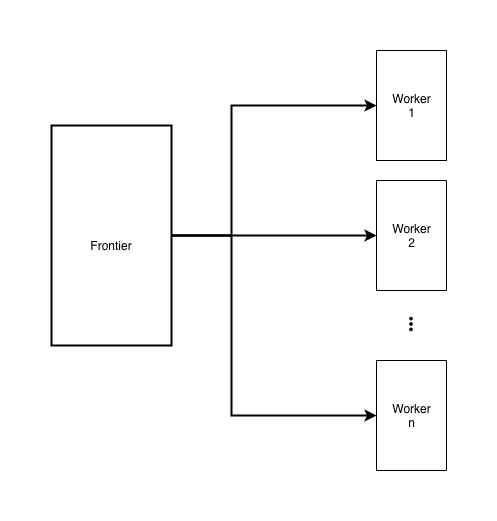
\includegraphics[width=0.9\textwidth]{jittered-delay.png}
		\caption{v.1.0 of the worker with a simultaneous access to the global frontier.}
		\label{fig:1}
	\end{minipage}\hfill
	\begin{minipage}{0.45\textwidth}
		\centering
		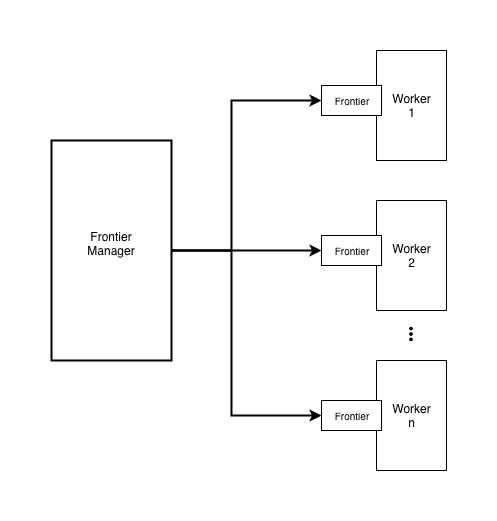
\includegraphics[width=0.9\textwidth]{frontier-manager.png}
		\caption{v2.0 of the worker with a \textit{Frontier Manager} which delegates the workload.}
		\label{fig:2}
\end{minipage}
\end{figure}


\section{Data Analysis}

\subsection{Experiment 1 - Provided seed all data}
\subsection{Experiment 2 - Extended seed all data}
~\ref{tab:1}

\begin{table}[hbt!]
	\centering
		\begin{tabular}{P{0.15\linewidth}|c|c}
			& Original seed & Extended seed \\ \hline
			running time [min] & 618 & 686  \\ \hline
			avg wait time [min] & 111.057 & 119.629 \\ \hline
			avg load time [ms] & 1351.347 & 1759.769 \\ \hline
			sites      & 288 & 327 \\ \hline
			pages      & 38268 & 58060 \\ \hline
			duplicates & 971 & 1766 \\ \hline
			links & 1585648 & 2569510 \\ \hline
			images     & 94368 & 187924 \\ \hline
			avg images  per page  & 6.3567 & 8.520 \\ \hline
			duplicate images & 64638 & 155277 \\ \hline
			data       & 28721 & 44761 \\ \hline
			avg data  per page    & 4.9853 & 6.170 \\ \hline
			duplicate data &11688 & 12593\\ \hline
			doc & 32 & 226 \\ \hline
			docx & 2 & 132 \\ \hline
			pdf & 230 & 941 \\ \hline
		\end{tabular}
	\caption{General statistics}
	\label{tab:1}
\end{table}

\begin{figure}
	\begin{minipage}{0.45\textwidth}
		\centering
		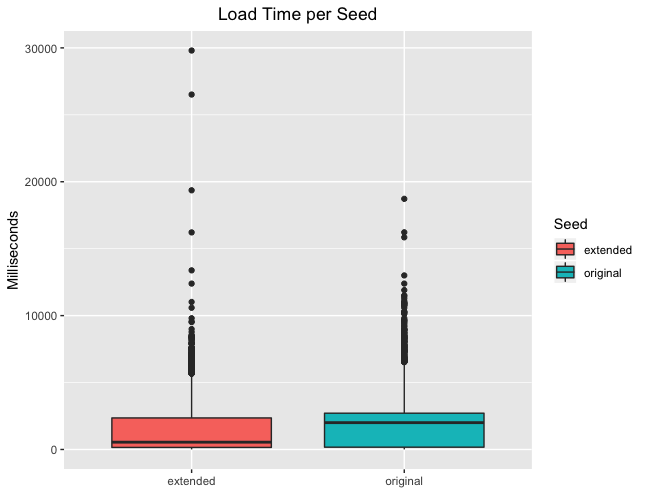
\includegraphics[width=0.9\textwidth]{load_time.png}
		\caption{Load time.}
		\label{fig:3}
	\end{minipage}\hfill
	\begin{minipage}{0.45\textwidth}
		\centering
		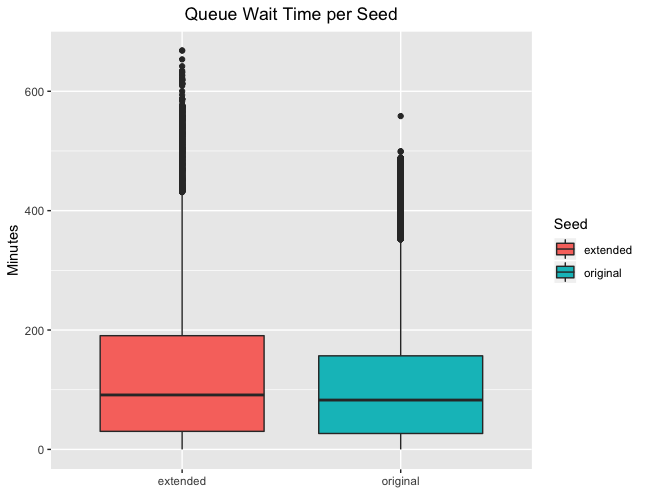
\includegraphics[width=0.9\textwidth]{queue_wait_time.png}
		\caption{Queue wait time.}
		\label{fig:4}
	\end{minipage}
\end{figure}

\section{Conclusion}

% SELECT count(*), clock_timestamp() FROM page;
% SELECT count(*), clock_timestamp() FROM link;
% SELECT count(*), clock_timestamp() FROM image;
% SELECT count(*), clock_timestamp() FROM page_data;

\bibliographystyle{IEEEtran}
\bibliography{refs}

\end{document}
